\documentclass[12pt]{article}


\usepackage{graphicx}
\graphicspath{{images/}}

\usepackage{hyperref}
\hypersetup{colorlinks=true, citecolor=blue, linkcolor=blue, urlcolor=blue}

%\usepackage{subcaption}

\usepackage[font=scriptsize, labelfont=bf]{caption}


\usepackage{sectsty}
\sectionfont{\normalsize}
\subsectionfont{\small}
\subsubsectionfont{\small}

\title{\large \textbf{How I Installed SPDROOT In Ubuntu 22.04 LTS OS}}

\author{Rishav Pandey\\ rishav160999@gmail.com}

\date{05.10.2022}

\begin{document}

\maketitle

\section{Installation of SPDROOT in Ubuntu 22.04 LTS}
In this article I'm going to talk about how I installed SPDROOT in my ubuntu 22.04 OS. At first, I was exactly following the installation guide present in NICA Gitlab repository. So, during the installation of FairSoft version jun19p2, I faced many errors, like ``pythia6 could not be created. Multiple definitions found", ``Geant4 could not be created" and many more. However, I resolved almost all of them in sequence but at last there was some error which pushed me install another version of FairSoft. I switched to FairSoft version apr21p2 and fortunately, I was able to install this without any error.\\

Then, I moved to install FairRoot v18.2.0 which is mentioned in NICA Gitlab repo. I was not able to configure the FairRoot, so I tried to install the same without doing ``git checkout v18.2.0". So, I think this installed the latest version of FairRoot in my PC and not the ``18.2.0".\\

After FairSoft and FairRoot was successfully installed, I started my installation of SPDROOT from master branch. Again, during the installation of SPDROOT, I faced configuration error like ``Looking for boost, couldn't find boost". So, in this case also I tried to install the same from another branch. I cloned another version of SPDROOT and did git checkout dev-hlit. Fortunately, this version was successfully installed, but during its installation, it complained that your FairRoot has no file named ``FairMCTracks.h".
So, I searched the same file in FairRoot github repo (under version 18.2.0), and manually added it in my FairRoot in the same path where it was complaining. Now, the manually added file needed to be compiled, so I did some changes in CMakeLists.txt and LinkDef.h file associated with its path. With this I was done with the installation of SPDROOT.\\

After all these when I tried to run an example (under macro folder), I was getting errors like ``unknown type name `SpdMCAegParticleProducer' " as shown in fig. \ref{Missing file error}. So, I tried to search for this file, and found that there are many files missing from my SPDROOT. Then I compared SPDROOT from master branch and SPDROOT from ``dev-hlit". And yes there were many missing files in later, including the one specified above. Manually adding files and compiling again and again could be a bad idea. Even I tried this, but there were many errors.\\


\begin{figure}[h]
\centering
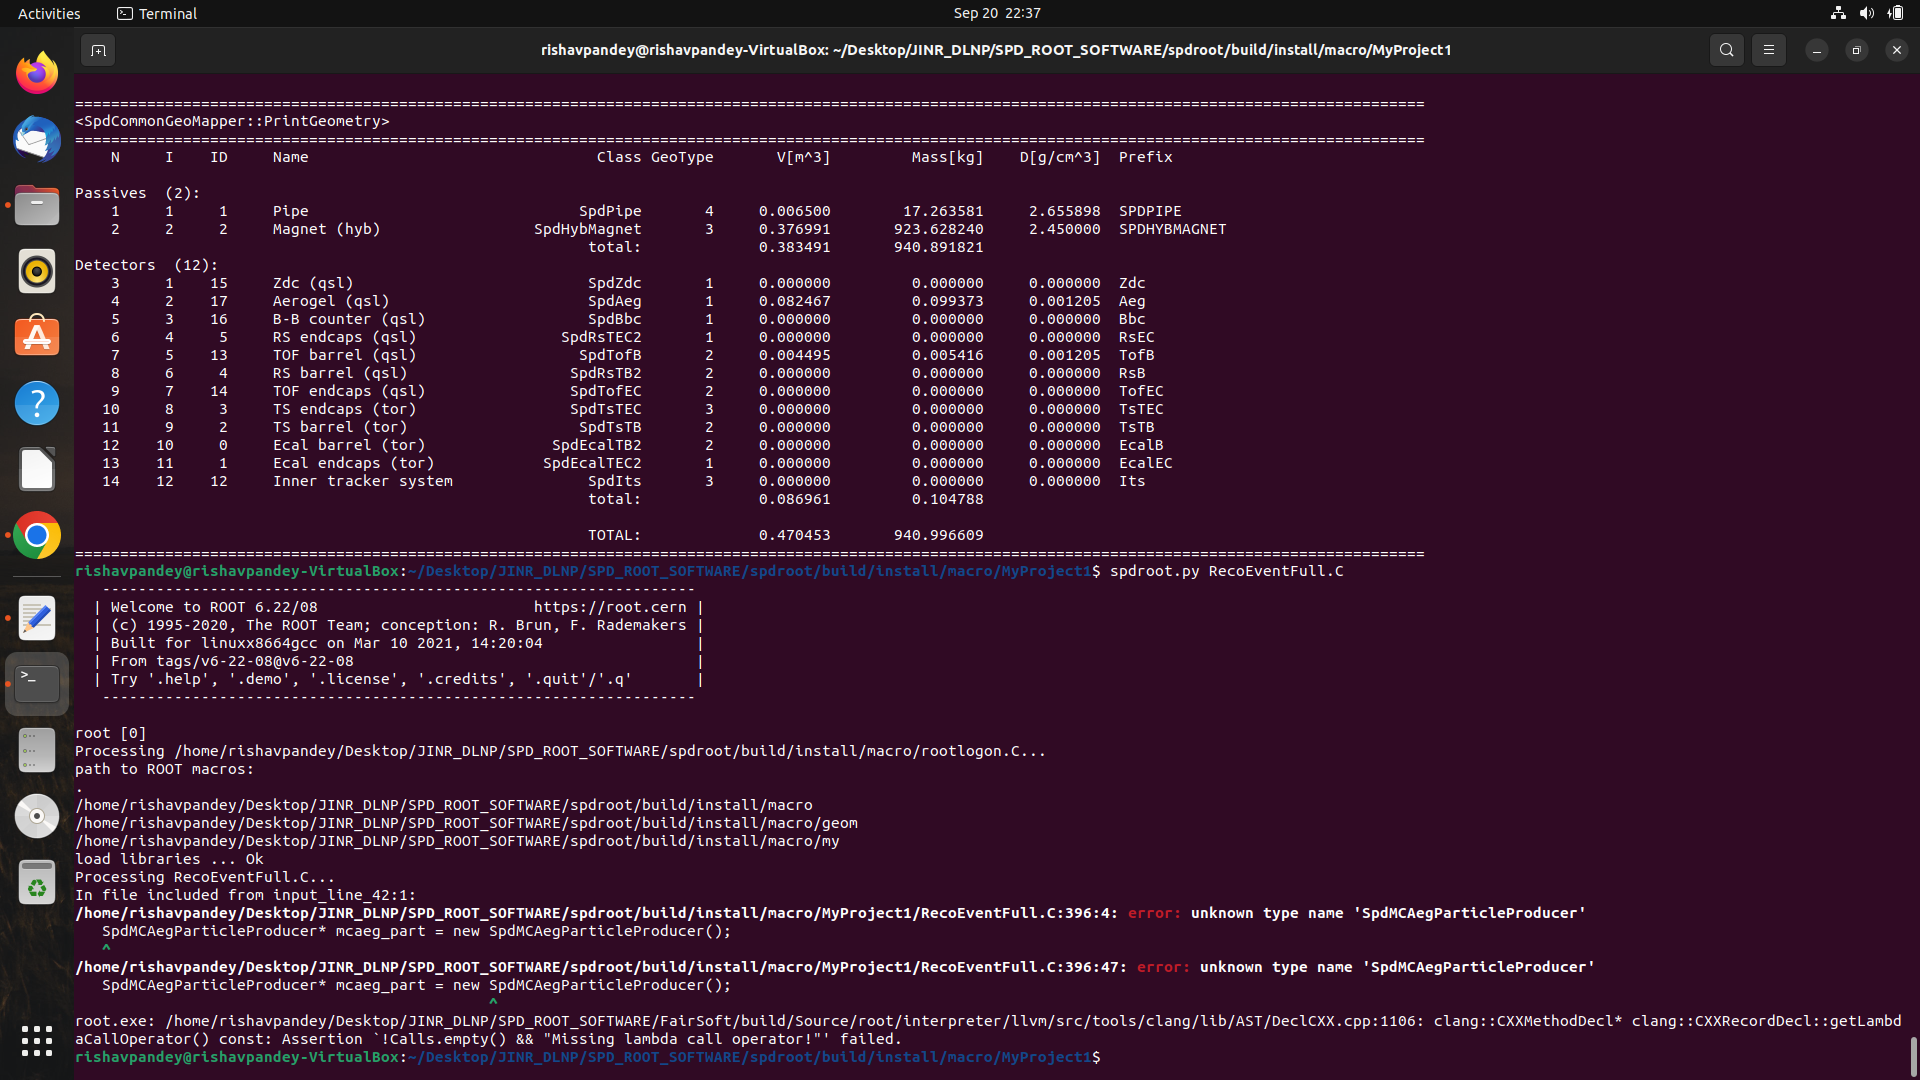
\includegraphics[scale=0.18]{ss1.png}
\caption{Missing file error}
\label{Missing file error}
\end{figure}

So, I tried a different approach. At first I cloned the SPDROOT from master branch only (because it has all required files, and there will be no error regarding file missing). Then, I configured this SPDROOT with the CMakeLists.txt copied from SPDROOT(dev-hlit).
This means that I was using SPDROOT from main branch but CMakeLists.txt was from `dev-hlit' version. I did this because the later was successfully installed (but complained many missing files). Now, with this combination I should have all files with successful installation of SPDROOT. And yes, this combination worked for me. Installation was successful. I was able to run the examples. But, my work went in vain when I tried to run the analysis script of my project. There was a complain, and it was ``The sink does not exist to store persistent branches".\\

I tried to look for solution online, but couldn't find any. However, I noticed that my SPDROOT uses the tree named `cbmsim' instead of 'spdsim'. So, I found that in my SPDROOT the `config' directory was not built during the installation. The reason was because I was using CMakeLists.txt from another version which uses cbmsim only and hence there was no command mentioned in the CMakeList to build that `config' directory. Hence, in that CMakeList I only added a line ``Install(DIRECTORY config DESTINATION .)" [please see fig. \ref{Code to build config directory}] and then compiled my SPDROOT again, and this time it built that `config' directory under the `install' directory. So, my SPDROOT started to use `spdsim' but the error ``The sink does not exist to store persistent branches" was still there.\\

\begin{figure}[h]
\centering
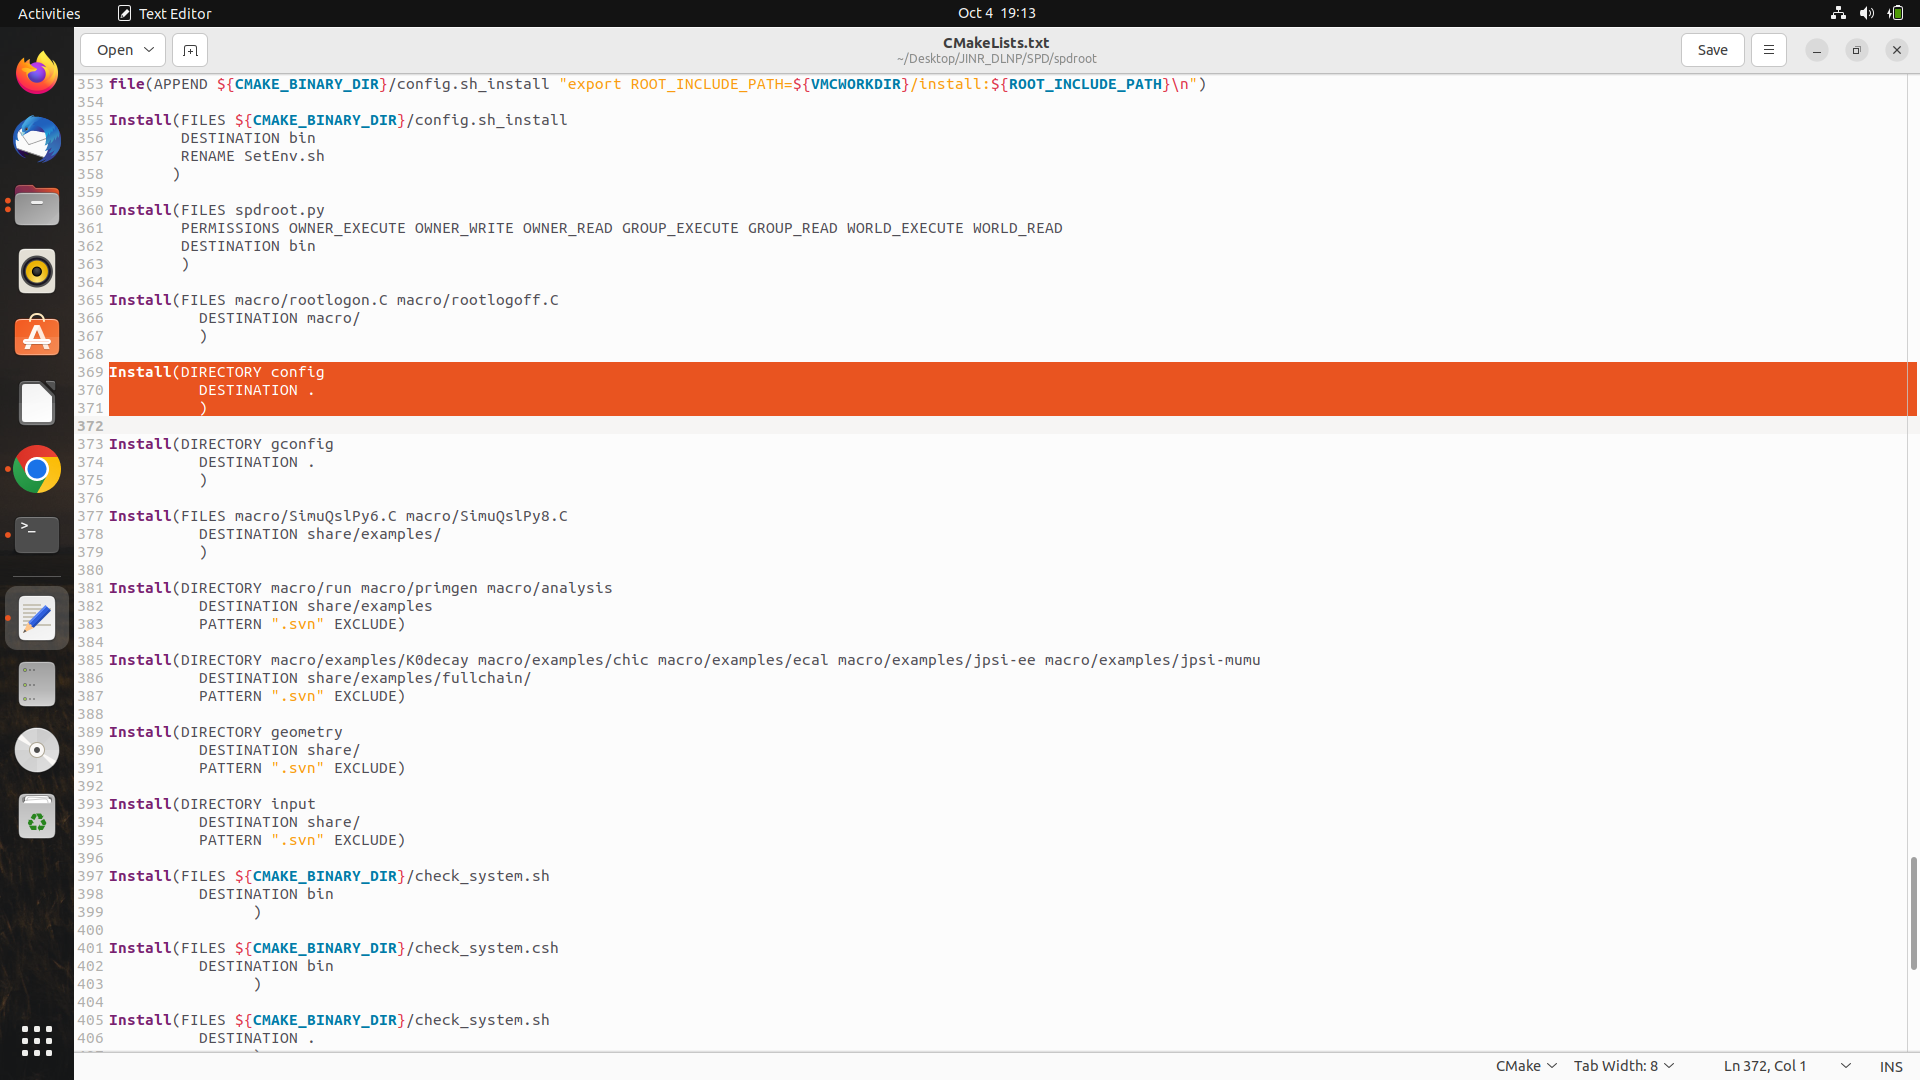
\includegraphics[scale=0.18]{ss5.png}
\caption{Code to build config directory}
\label{Code to build config directory}
\end{figure}

I tried to search this string ``The sink does not exist to store persistent branches" using `grep' and found that the error was coming from `FairRootManager.h' which was inside FairRoot. Then I compared the FairRootManager.h of my latest version of FairRoot with the FairRootManager.h present in older version which was recommended to install. I found a small change between those two files. As shown in fig. \ref{Comparing FairRootManager.h between latest version (shown left) with v18.2.0 (shown right)}, there is no conditional statement in older version whereas in latest version there is. So, I followed the older version and removed that conditional statement. Compiled FairRoot and SPDROOT followed by installation removed the error. With this my SPDROOT was/is working fine. Also, I completed my project in both the versions of SPDROOT and compared the results/plots obtained. There is almost no difference.\\

\begin{figure}[h]
\centering
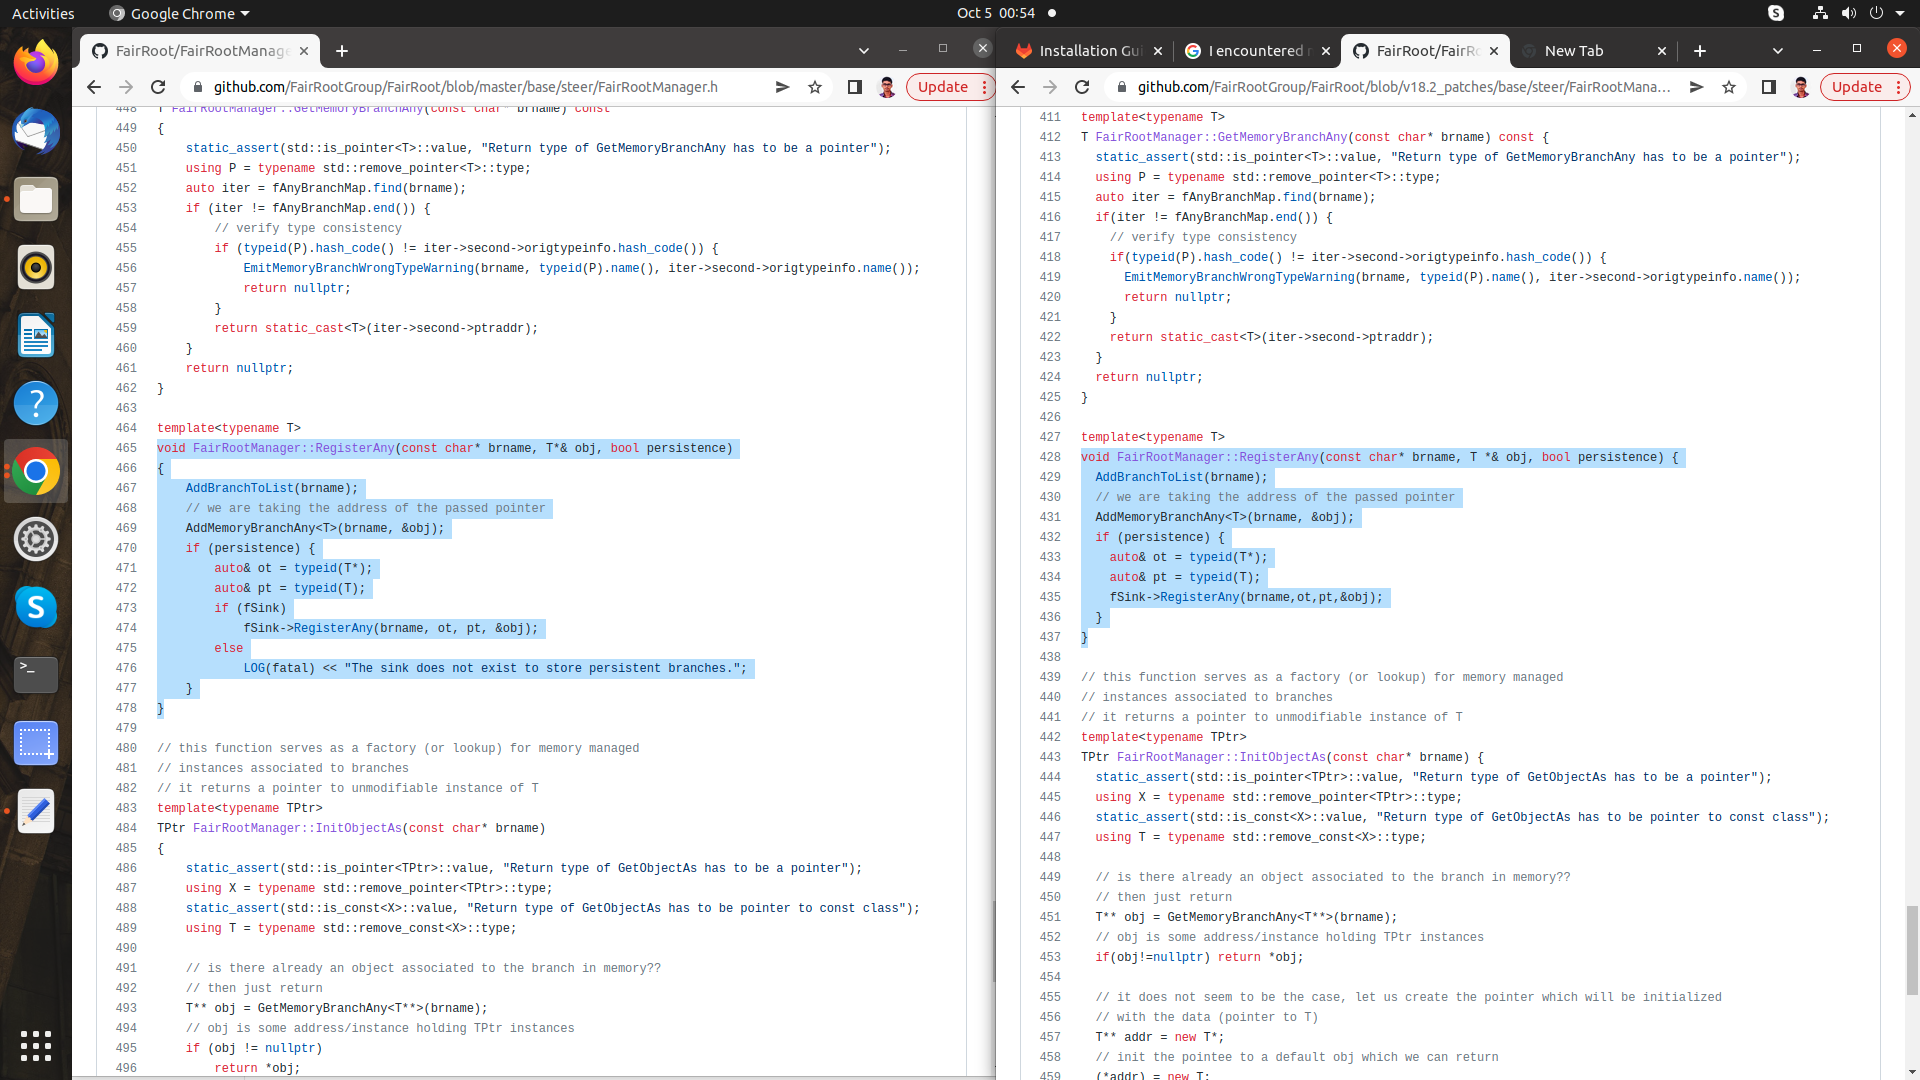
\includegraphics[scale=0.18]{ss3.png}
\caption{Comparing FairRootManager.h between latest version (shown left) with v18.2.0 (shown right)}
\label{Comparing FairRootManager.h between latest version (shown left) with v18.2.0 (shown right)}
\end{figure}

But later on I came to know that although my SPDROOT is working fine and producing output, but one of its feature `DisplayEvent.C' doesn't work and upon running there was an error ``no member named `SetInputFile' in `SpdRunAna' [Please see fig. \ref{Missing function SetInputFile}]". On probing I came to know the error was again due to the latest version of FairRoot which I was using and it was due to file named `FairRunAna'. I did comparison of this file in both the versions and found that SetInputFile function is missing in latest version which is required to run DisplayEvent.C. I manually added its definition and code in .h and .cxx file respectively as shown in fig. \ref{Adding SetInputFunction in .cxx (left) and .h (right) files, so that DisplayEvent.C could run}. Compiled and installed both FairRoot and SPDROOT again, and the error vanished. It's working now and I'm happy.\\

\clearpage

\begin{figure}[h]
\centering
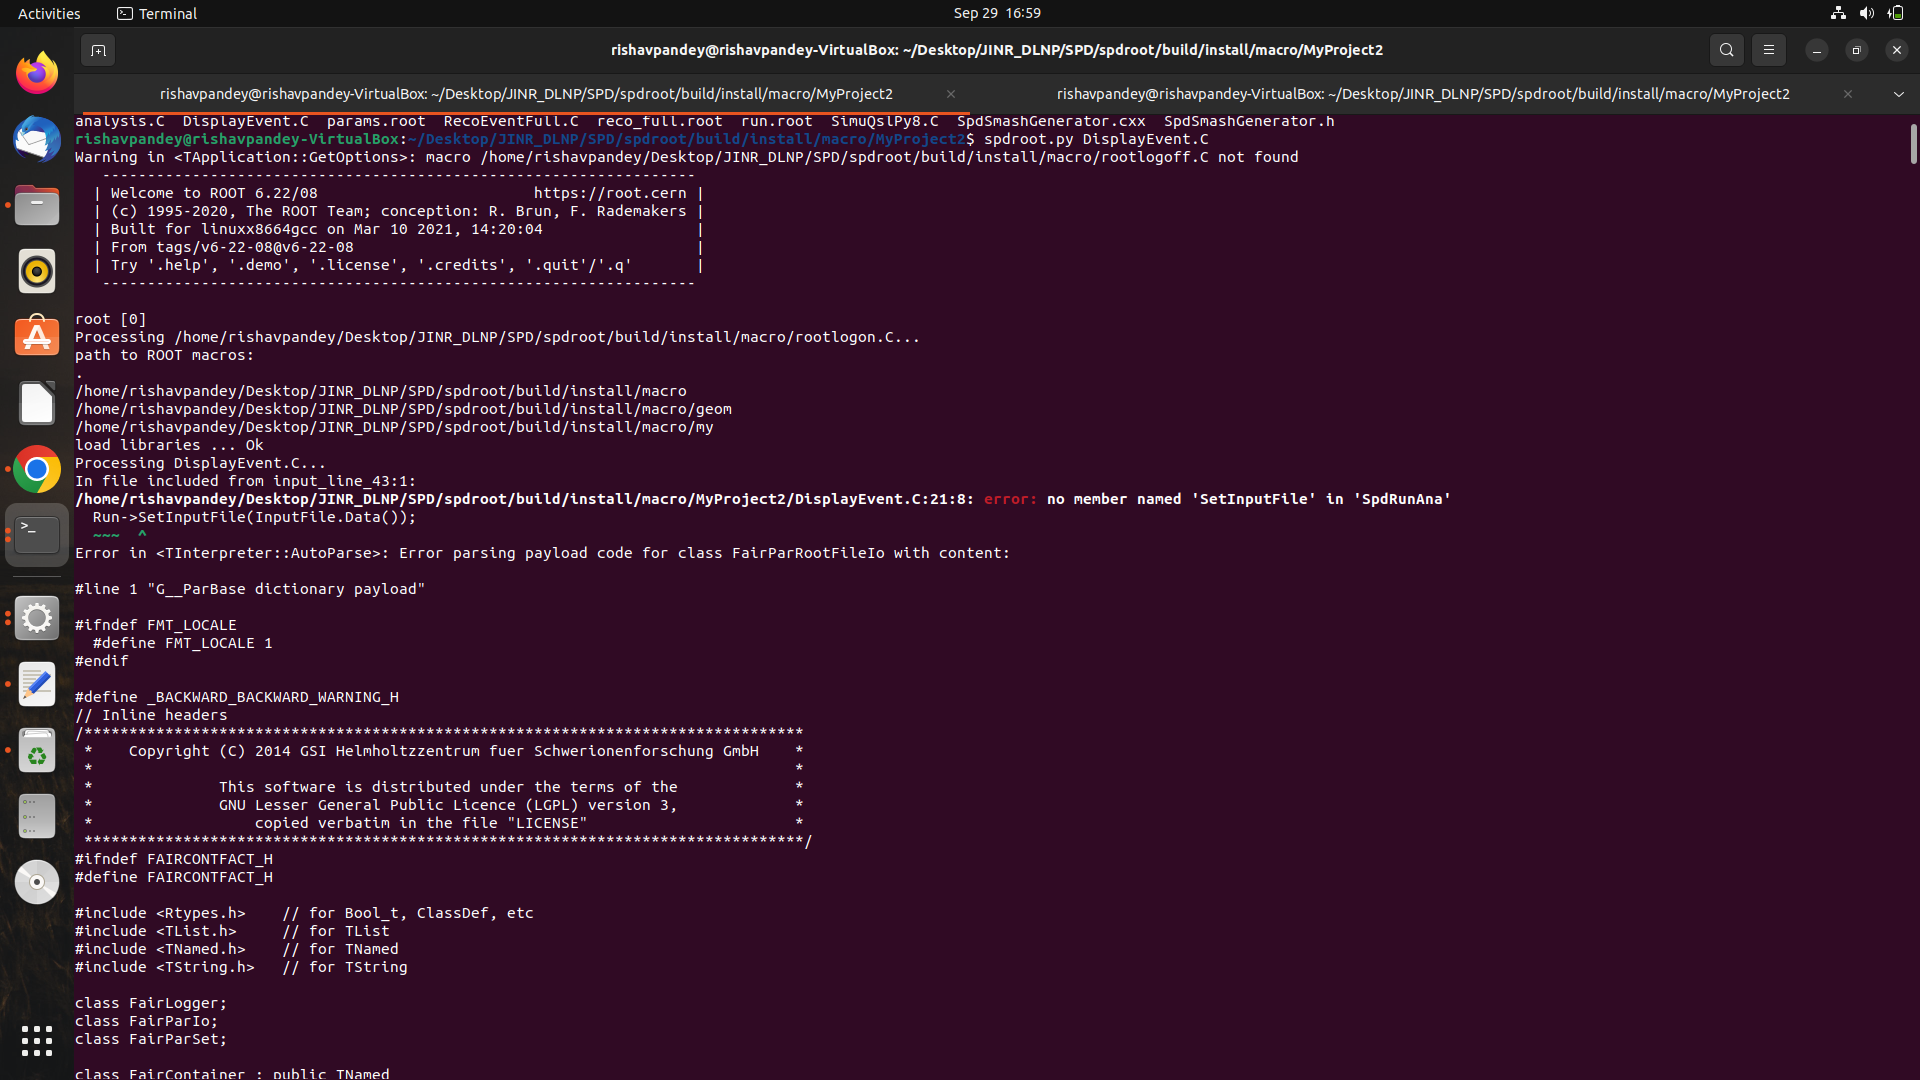
\includegraphics[scale=0.165]{ss4.png}
\caption{Missing function SetInputFile}
\label{Missing function SetInputFile}
\end{figure}

\begin{figure}[h]
\centering
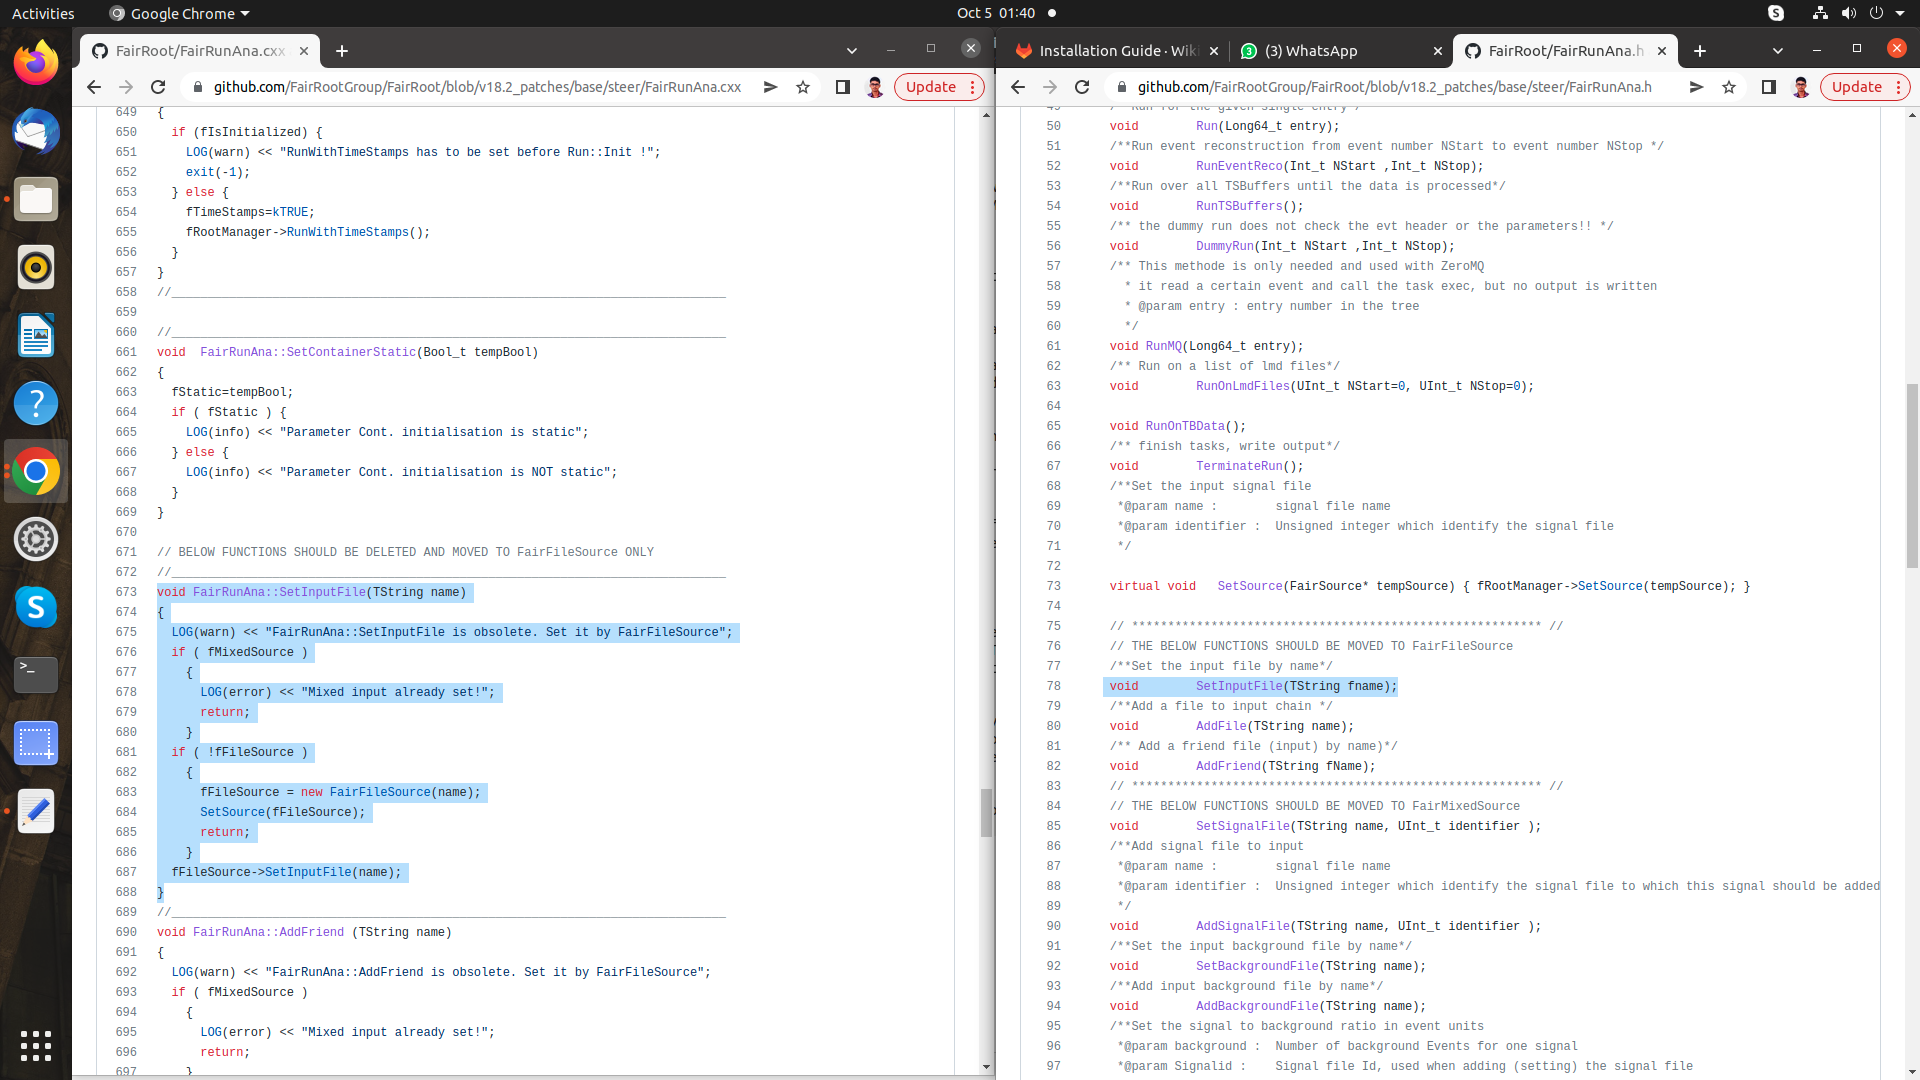
\includegraphics[scale=0.165]{ss2.png}
\caption{Adding SetInputFunction in .cxx (left) and .h (right) files, so that DisplayEvent.C could run}
\label{Adding SetInputFunction in .cxx (left) and .h (right) files, so that DisplayEvent.C could run}
\end{figure}

Thank you for reading :)

\end{document}